% !TEX root = ../main.tex
\graphicspath{ {./figures/} }

%%%%%%%%%%%%%%%%
\chapter{Design}
\label{sec:design}
%%%%%%%%%%%%%%%%

This section describes our implementation of liquid democracy with fractional delegation. We start by introducing the problem, then introducing prerequisite definitions and finally the method to resolve delegations. 

\section{Problem Statement}

We consider a fractional delegation model, where voters may distribute their vote across multiple  delegates. Each voter can either retain their full vote or delegate it to others in fractional amounts summing to one.

We pose the following problem.

\begin{enumerate}
\item \textbf{Given} a set of voters and their delegations, where each voter has one vote, and either:
\begin{enumerate}
\item votes directly, or 
\item delegates their vote such that their vote is delegated to other delegates in its entirety
\end{enumerate}
\item \textbf{We want to find} the final voting power of each voter ("resolve the delegation graph") such that:
\begin{enumerate}
\item a voter's final voting power is zero if they choose to delegate and not vote directly 
\item a voter's final voting power is equal to the amount of votes delegates to them, including transitive delegations, otherwise
\item the sum of the final power of all nodes must be equal to the amount of votes initially in the graph
\end{enumerate}
\end{enumerate}

\section{Implementing Liquid Democracy with Fractional Delegation}
\label{sec:ld_with_frac_del}

\subsection{Definitions}

\textbf{Delegation graphs} represent \textbf{delegations} between voters using weighted, directed edges between nodes. \textbf{Power} refers to a fractional amount of votes. Each node initially has one vote, or an \textbf{initial power} $p^{(0)}_v = 1$. Each delegation between two nodes has a positive, nonzero \textbf{weight} $w \in \mathbb{R}^+$. \textbf{Resolving delegations} means to determine how much power each sink holds according to the delegations. After resolving delegations, a node $v \in V'$s \textbf{final power}, is $p_v \in \mathbb{R}_{\ge0}$. A more rigid definition of a nodes final power will be introduced in section XX.

As per the problem statement, voters are strictly given the choice to either delegate their vote (fractional) in its entirety, or vote directly. The electorate is thus divided into two disjoint \textbf{sinks} S, who actually vote, and \textbf{delegators} D. 

We thus define a \textbf{delegation graph} as a finite, directed, weighted graph $G = (V, E)$, with sinks $S$ and delegators $D$ as follows:

\begin{enumerate}
\item $V = S \dot\bigcup D$, meaning that $V$ is the union of the two disjoint sets of sinks and delegators.
\item Each $e \in E$ is a triple $(u, v, w)$, denoting a delegation from node $u$ to node $v$ of weight $w$.
\item Each sink $s \in S$ has no outgoing edges.
\item Each delegator $d \in D$ has $n \in \mathbb{N}^+$ outgoing edges, each with a positive weight \footnotemark, such that the sum of all of its outgoing edge weights equals 1.
\item Each voter $v \in V$ has corresponding power value, which is initially 1.
\end{enumerate}

\footnotetext{Edge weights should not be 0, since the edge should be entirely omitted in this case.}

 \subsection{Conservation of Power}
 
 A vital property we set for the delegation graph is the conservation of power. While some authors have experimented with implementations of liquid democracy where this is not the case \cite{bersetcheGeneralizingLiquidDemocracy2022, boldiViscousDemocracySocial2011}, we believe that for a system to be truly democratic, we must assert delegating is not penalised, so a vote cast by a sink should not be different in value to a vote cast by a sink through delegation from a delegator. Thus, any implementation needs a mechanism to ensure that the sum of the final power of all sinks is equal to the sum of the initial power of all nodes.

\subsection{Closed Delegation Cycles}

We define a \textbf{closed delegation cycle} $C \subseteq V$ in a delegation graph $G = (S \dot\bigcup D, E)$ as a cycle in $G$ such that for every node $v \in C$, there exists no path from $v$ to any sink node in $S$. That is,
\[
\forall v \in C,\ \nexists\ \text{path from } v \text{ to any } s \in S.
\]

\begin{figure}[t]
    \centering
    \begin{subfigure}[t]{0.32\textwidth}
        \centering
        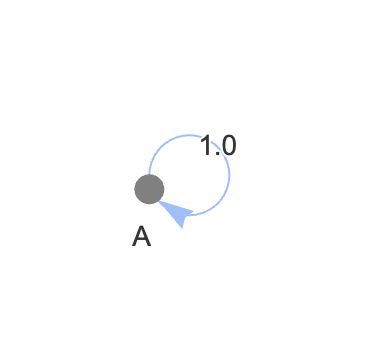
\includegraphics[width=\textwidth]{invalid_graph_1}
    \end{subfigure}
    \hfill
    \begin{subfigure}[t]{0.32\textwidth}
        \centering
        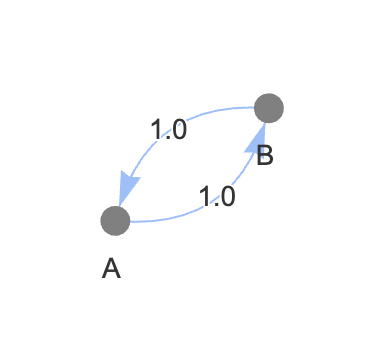
\includegraphics[width=\textwidth]{invalid_graph_2}
    \end{subfigure}
    \hfill
    \begin{subfigure}[t]{0.32\textwidth}
        \centering
        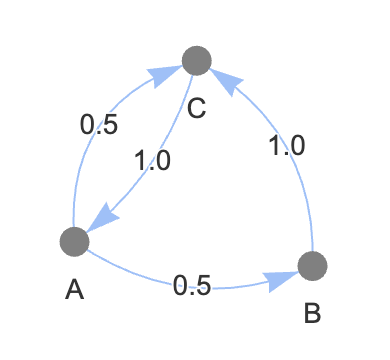
\includegraphics[width=\textwidth]{invalid_graph_3}
    \end{subfigure}
    \caption{Closed delegation cycles}
    \label{fig:closed-delegation-cycles}
\end{figure}

\Cref{fig:closed-delegation-cycles} shows exemplary closed delegation cycles. These cycles lead to contradictory situations, as power delegated within never reaches a sink. Some works discuss ways to handle power stuck in such cycles or mitigate the risk of such cycles appearing, but effectively it is lost. \cite{behrensCircularDelegationsMyth2015, brillInteractiveDemocracy2018} This means that none of the nodes in a closed cycle will vote, which is in line with the will of voters, who all wish to not vote themselves, instead delegate their power, letting their delegate(s) decide what to do with this power. 

In practice, such cycles need to be addressed before resolving delegations. Our approach to this is to find all such cycles, and collapse them into an additional sink node in the graph, the \textbf{cycle sink node}. Any delegation into the cycle is redirected into the cycle sink node,  thus ensuring the graph no longer has any closed delegation cycles. The algorithm to do so can be found in annex XX. \TODO{Add this into the annex, if that necessary...} 

We prove below, that given the absence of such closed delegation cycles, delegations are resolvable given a delegation graph. 

\begin{theorem}
Let $G = (S \dot\bigcup D, E)$ be a delegation graph. If $G$ contains no closed delegation cycles, then for every delegator $d \in D$, there exists a path from $d$ to a sink node $s \in S$.
\end{theorem}
\begin{proof}
Suppose, for contradiction, that $G$ contains no closed delegation cycle, but $\exists d \in D$ such that no path from $d$ leads to any sink $s \in S$. Since G is a finite graph, any walk from $d$ must eventually repeat nodes, implying a cycle. If at least one node in this cycle can reach a sink, there would be a path for all others in the cycle to reach a sink via this node as well, thus all nodes in the cycle can not reach a sink either. Thus, G does contain a closed delegation cycle. $\lightning$
\end{proof}

 A \textbf{well-formed delegation graph} G is defined as a delegation graph, which contains no closed delegation cycles. Note, that while a self loop of weight one is not allowed in a well-formed delegation graph, a self loop of weight $w \le 1$ is allowed as long as the rest of the node's power eventually flows to a sink. Since a delegator can't vote, any power a delegator delegates to themselves will "flow" back into the node, and then be redistributed to the nodes delegates. 

\section{Resolving Delegations}

\begin{figure}[t]
	\centering
	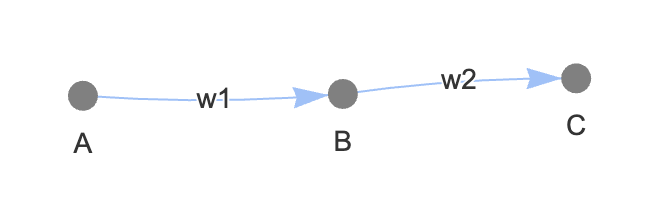
\includegraphics[width=0.4\textwidth]{delegation_graph_sample}
	\caption{Sample delegations}
	\label{fig:sample_delegations}
\end{figure}

Sink node $C$ receives its own initial vote, and is also delegated a fraction $w_2$ of $B$'s vote. Node $B$, in turn, receives its own vote and a fraction $w_1$ of A's vote. Let $p'_A$ and$ p'_B$ denote the \textbf{standing power} of nodes $A$ and $B$, i.e. the total amount of power delegated to them. Then, the final power of $C$, assuming no other incoming delegations, is:

\[
p_C = 1 + w_2p'_B = 1 + w_2(1 + w_1p'_A)
\]

This motivates the recursive definition of standing power in a delegation graph $G = (V, E)$ as:

$p'_v = 1 + \sum_{(u, v, w) \in E} wp'_u$

Using this, we define the final voting power $p_v$ of a node as:

\[
p_v = 
\begin{cases}
 p'_v, v \in S \\ 
 0, v \in D 
 \end{cases}
\]

The problem of finding each node's standing power is thus a problem of solving a system of linear equations, namely calculating the standing power for all nodes. We can prove, that given a well-formed delegation graph, this method returns a unique solution, and that given a well formed delegation graph and the above definition of the final power of a node, power is conserved.

1. power is conserved

2. there is a unique solution when the graph is well formed?

\subsection{Existence of a Unique Solution}

\TODO{There are two ways I can prove this. Firstly is to just quote (p.74-76). Alternatively, a more complicated but less weird source would be to prove this shit using (theore 8.1.26 and some other theorem, see chatgpt Chat "Trace behavior of matrices"). the second one I am not 100\% convinced yet that it actually works}

first link \url{file:///Users/DavidHolzwarth/Downloads/978-1-84996-299-5.pdf} (Max-Linear Systems: Theory and Algorithms) by Butkovic

second link \url{https://www.anandinstitute.org/pdf/Roger_A.Horn.%20_Matrix_Analysis_2nd_edition(BookSee.org).pdf}

 \subsection{Conservation of Power}
 
 In order to assure that the power is conserved during delegation, it may seem intuitive to add a constraint $\sum_{s \in S} p_s = |V|$ to the system of linear equations. However, we prove that such an equation is not strictly necessary, as the other equations in the system of equations already imply the conservation of power.

We start with the solutions $\{p'_v | v \in V\}$.

\begin{align*}
\forall v \in V: p'_v &= 1+\sum_{(u, v, w) \in E} \bigl(wp'_u \bigr) \\
\implies \sum_{v \in V} p'_v &= \sum_{v \in V} \bigl( 1 + \sum_{(u, v, w) \in E} \bigl( wp'_u \bigr ) \bigr) \\
&= \sum_{v \in V} 1 + \sum_{v \in V} \sum_{(u, v, w) \in E} wp'_u \\
&= |V| + \sum_{v \in V} \sum_{(u, v, w) \in E} wp'_u \\
&= |V| + \sum_{(u, v, w) \in E} wp'_u
\end{align*}

Focusing on the $\sum_{(u, v, w) \in E} wp'_u$ term, this can be re-grouped by $u$ as follows 

\begin{align*}
\sum_{(u, v, w) \in E} wp'_u &= \sum_{u \in V} \sum_{(u, v, w) \in E} wp'_u \\
&= \sum_{u \in V} p'_u  \sum_{(u, v, w) \in E} w
\end{align*}

Since, according to our definition of a delegation graph, all sinks have no outgoing notes, and all delegators's outgoing node weights add up to 1, we know that

\[
\sum_{(u, v, w) \in E} w = \begin{cases} 1, u \in D \\ 0, u \in S \end{cases}
\]

Thus, we can rewrite the above equation.

\begin{align*}
\sum_{u \in V} p'_u  \sum_{(u, v, w) \in E} w &= \left(\sum_{u \in D} p'_u  \sum_{(u, v, w) \in E} w \right) + \left( \sum_{u \in S} p'_u  \sum_{(u, v, w) \in E} w \right) \\
&= \left( \sum_{u \in D} p'_u \cdot 1 \right) + \left(\sum_{u \in S} p'_u \cdot 0 \right) \\
&= \sum_{u \in D} p'_u
\end{align*}

Focusing now on term $\sum_{v \in V} p'_v$, since $V = S \bigcup D$ , and $S$ and $D$ are disjunct we can say

\[
\sum_{v \in V} p'_v = \sum_{v \in S} p'_v  + \sum_{v \in D} p'_v 
\]

Thus, these two equations, we get

\[
\sum_{v \in S} p'_v  + \sum_{v \in D} p'_v  = |V| + \sum_{u \in D} p'_u
\]
\[
\implies \sum_{v \in S} p'_v   = |V| \qed
\]


\subsection{Resolving Delegations by Solving a System of Linear Equations}

With the insights gained in the previous sections in mind, it is now possible to formulate the following method to resolving delegation graphs.

\begin{enumerate}
\item Set up a system of linear equations, such that for each node $v \in V$ there is an equation $p'_v = 1+\sum_{(u, v, w) \in E}wp'_u$
\item Solve the system of linear equations to find the value of $p'_v$ for all $v \in V$
\item For each $s \in S$ set $p_s = p'_s$
\item For each $d \in D$ set $p_d = 0$
\end{enumerate}

